\chapter{Wavelets}
\label{app:wavelet}

\section{Introduction}
In the previous chapter, the \gls{fft} has been briefly described. It maps $N$ time-domain datapoints into $N$ frequency-domain datapoints. The \gls{fft} retain the information about the original signal, expressing it in the frequency domain. In other words, the \gls{fft} does not retain any knowledge about the time evolution of the signal and preserves the number of datapoints.

Another tool for signal processing is the wavelet. There are two main categories:
\begin{itemize}
\item  Wavelet Transform (\gls{wt}), which maps the datapoints of a 1D signal into a 2D plane, giving information about the frequency content of a signal at a given time.
\item Wavelet Packet Decomposition (\gls{wpd}), which is a tool that allows to decompose a signal into a tree of sub-bands, down-sampled signals. 
\end{itemize}

A mother wavelet is a function that complies with the following conditions:
\begin{align}
\int_{-\infty}^{\infty} \psi(t) dt = 0 & \qquad &\text{\gls{ie} it has a mean value of zero.} \\
\int_{-\infty}^{\infty} |\psi(t)|^2 dt = 1 & \qquad &\text{\gls{ie} it has a unitary energy.}
\end{align}

For example, the Morlet wavelet is a complex wavelet, which complies with the above conditions. It is defined as:
\begin{equation}
\psi(t) = \frac{1}{\sqrt{\pi f_b}} e^{i 2 \pi f_c t} e^{-t^2/f_b} =  \frac{1}{\sqrt{\pi f_b}}[ \cos(2 \pi f_c t) + j\cdot \sin(2 \pi f_c t)] e^{-t^2/f_b}
\end{equation}
where $f_c$ is the central frequency and $f_b$ is the bandwidth. The Morlet wavelet is a complex wavelet, which means that it has a real and an imaginary part, as shown in Figure \ref{fig:morlet}. 

\begin{figure}
\centering
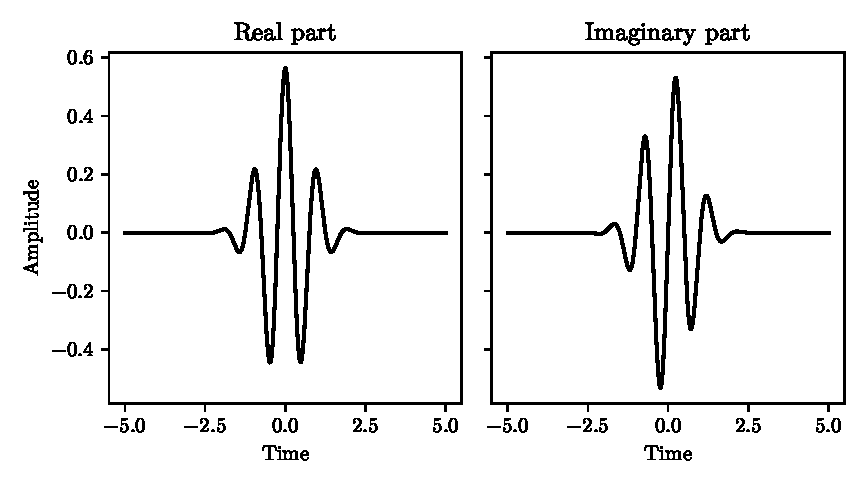
\includegraphics[]{images/morlet.pdf}
\caption{Real and imaginary part of the Morlet wavelet}
\label{fig:morlet}
\end{figure}

\section{Scaling and translation}
The wavelet is a function of time, and it can be scaled and translated. The scaling allows to investigate the frequency content of the signal, while the translation allows to investigate the time evolution of the signal.

So a general wavelet is obtained by scaling and translating a mother wavelet:
\begin{equation}
\psi_{a,b}(t) = \frac{1}{\sqrt{a}} \psi \left( \frac{t-b}{a} \right)
\end{equation}
where $a$ is the scaling factor and $b$ is the translation factor. $\psi_{1,0}$ is the mother wavelet. Some wavelets are shown in Figure \ref{fig:wavelets}.

\begin{figure}
\centering
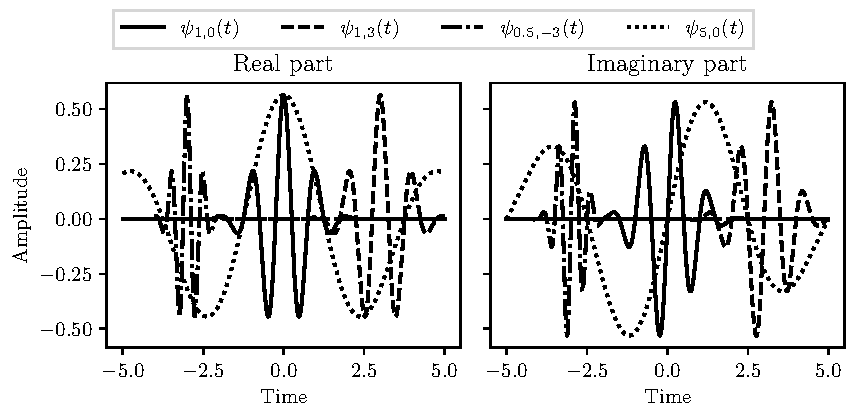
\includegraphics{images/morlet_trasl.pdf}
\caption{Effect of scaling and translation on the Morlet wavelet}
\label{fig:wavelets}
\end{figure}

\section{Wavelet Transform}
Intuitively, the \gls{wt} is a tool that allows to investigate the frequency content of a signal at a given time. The transform is defined as a function of the scaling and translation factors:
\begin{equation}
W(a,b) =\frac{1}{\sqrt{a}} \int_{-\infty}^{\infty} x(t) \psi \left( \frac{t-b}{a} \right)dt
\end{equation}
where $x(t)$ is the signal. The wavelet transform is a 2D plane, where one axis is the scaling factor and the other axis is the translation factor.

\section{Wavelet Packet Decomposition}
The \gls{wpd} is a tool that allows to decompose a signal into a tree of sub-bands, down-sampled signals. Each level is computed by the decomposition of the previous level, forming a binary tree \cite{akansu1991}. Being a binary tree, as shown in the \autoref{fig:wpd}, the number of sub-bands at level $n$ is $2^n$. The downsampling, done at each level, reduces the number of datapoints by a factor of 2, so the overall number of datapoints is preserved.

\begin{figure}
\centering
\includegraphics{images/wpd.pdf}
\caption{Wavelet Packet Decomposition tree}
\label{fig:wpd}
\end{figure}


At each stage, the signal is passed through a low-pass filter and a high-pass filter. The low-pass filter is used to compute the approximation coefficients, while the high-pass filter is used to compute the detail coefficients. The filters are finite impulse response filters, and the coefficients are computed by convolution. The decomposition is done recursively, until the desired level is reached.

Since this is just a transformation, the original signal can be reconstructed by the inverse wavelet packet decomposition. The reconstruction is done by upsampling the coefficients and passing them through the inverse filters.


\begin{figure}
\centering
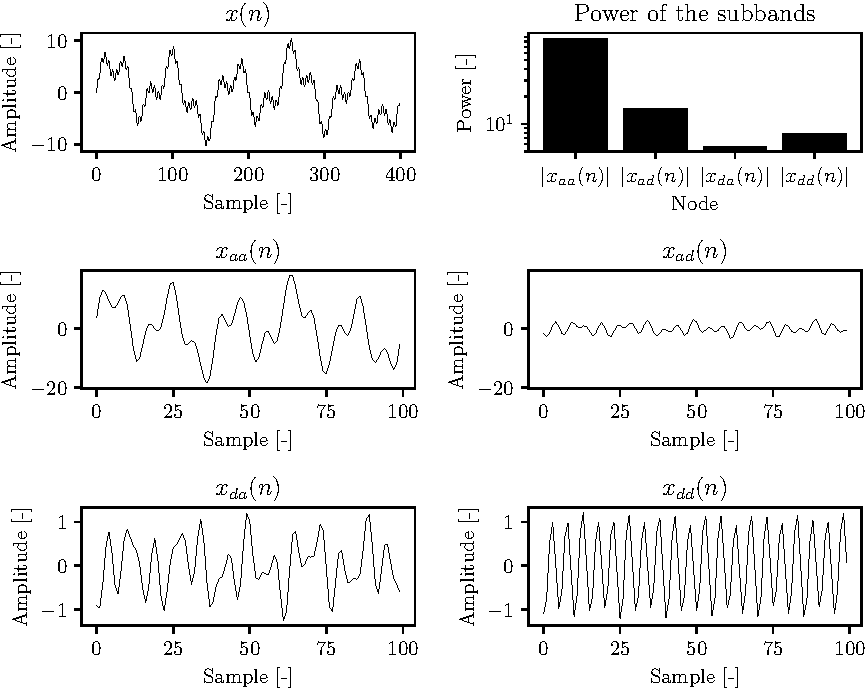
\includegraphics{images/WPD_result.pdf}
\caption{Wavelet Packet Decomposition of a signal using a tree of depth 2 to get 4 sub-bands}
\label{fig:wpd_result}
\end{figure}

As an example, the \autoref{fig:wpd_result} shows the result of the \gls{wpd} of a signal using a tree of depth 2 to get 4 sub-bands. The original signal is shown in the top left corner. In the top right corner, the norm of the coefficients is shown. The rest of the sub-bands are shown in the central and bottom rows. It's possible to see that $x_{aa}(n)$ is the approximation of the original signal, while  $x_{dd}(n)$ contains the high-frequency content of the original signal. 

The signals $x_{aa}(n)$, $x_{ad}(n)$, $x_{da}(n)$, and $x_{dd}(n)$ can be used to reconstruct exactly the original signal, using the inverse wavelet packet decomposition. For the purpose of this thesis, the \gls{wpd} is used to decompose the signals into sub-bands, and the coefficients $l^2$-norms are used as features for the \gls{ml} algorithms.